\documentclass[preview]{standalone}
\usepackage[caption=false,font=footnotesize]{subfig}
\usepackage[utf8]{inputenc}
\usepackage{ctex}
%graphics
\usepackage{tikz}

\begin{document}

\begin{figure}
\centering
\subfloat[{ 单稳态}] {
    \label{fig:monostable}
    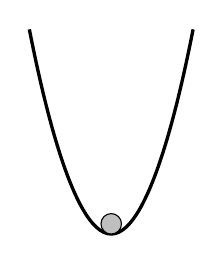
\begin{tikzpicture}[scale=0.65]
        \draw[very thick] (-1.6,2) parabola bend (0, -2) (1.6, 2);
        \draw[fill=gray!50] (0, -1.8) circle [radius=.2cm];
    \end{tikzpicture}
}
\hfil
\subfloat[{ 双稳态}] {
    \label{fig:bistable}
    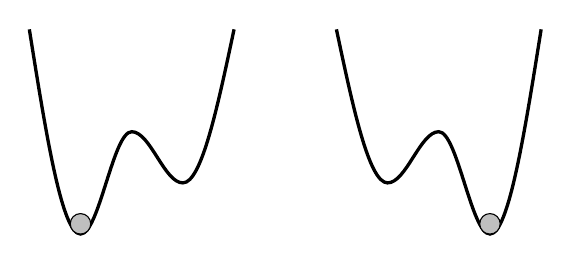
\begin{tikzpicture}[scale=0.65]
        \draw[very thick] (-5,2) sin (-4,-2) cos (-3.5,-1) sin (-3,0) cos (-2.5,-0.5) sin (-2, -1) cos (-1,2);
        \draw[fill=gray!50] (-4,-1.8) circle [radius=.2cm];
        \draw[very thick] (5,2) sin (4,-2) cos (3.5,-1) sin (3,0) cos (2.5,-0.5) sin (2, -1) cos (1,2);
        \draw[fill=gray!50] (4,-1.8) circle [radius=.2cm];
    \end{tikzpicture}
}
\end{figure}

\end{document}
